\documentclass{beamer}
\usetheme{Madrid}

\usepackage{amsmath}
\usepackage{graphicx}

\usepackage[justification=centering]{caption}
\usepackage{subcaption}

\usepackage{xurl}

% default path to images and other assets
\graphicspath{{assets/}}

% disable wrapping
\tolerance=1
\emergencystretch=\maxdimen
\hyphenpenalty=10000
\hbadness=10000

% number figure caption
\setbeamertemplate{caption}[numbered]

% display bib label in references
\setbeamertemplate{bibliography item}{\insertbiblabel}
\setbeamertemplate{bibliography entry title}{}
\setbeamertemplate{bibliography entry location}{}
\setbeamertemplate{bibliography entry note}{}

% Author name with matriculation number
% https://tex.stackexchange.com/questions/622753/how-to-format-a-beamer-title-with-two-names-and-one-institution
\newcommand{\aut}[2]{\parbox{30mm}{\centering #1 \\ #2}}

% Metadata
% ------------------------
\title[Instance segmentation]{Instance segmentation of biomedical images with an object-aware
embedding learned with local constraints}
\subtitle{Seminar Computational Life Science}

\author[Oleh Shkalikov]{\aut{Oleh Shkalikov}{5102818}}

\institute[TU Dresden]{TU Dresden, Computer Science Faculty}

\date{9 May, 2023}

% ------------------------

\begin{document}

\frame{\titlepage}

\begin{frame}
    \frametitle{Agenda}
    \tableofcontents
\end{frame}

\section{Problem formulation}

\begin{frame}
    \frametitle{Semantic VS instance segmentation}

    \begin{figure}[h]
        \begin{subfigure}{0.49\textwidth}
            \centering
            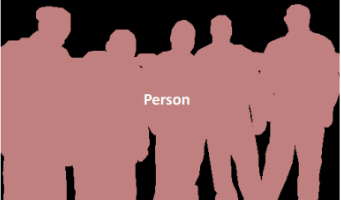
\includegraphics[width=0.8\textwidth]{semantic_segm_example.png}
            \caption{Semantic segmentation}
        \end{subfigure}
        \begin{subfigure}{0.49\textwidth}
            \centering
            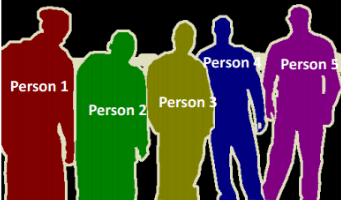
\includegraphics[width=0.8\textwidth]{instance_segm_example.png}
            \caption{Instance segmentation}
        \end{subfigure}
        \caption{Comparison of the different segmentation types. Source publication is \cite{segm_type_comp}}.
    \end{figure}

\end{frame}

\begin{frame}[allowframebreaks]
    \frametitle{References}

    \bibliographystyle{apalike}
    \bibliography{references.bib}
\end{frame}

\end{document}